\section{Supplementary native worked examples}\label{app:supp-native-examples}

This appendix collects the heavier native worked tables that support audit and reproduction while keeping the main examples compact. All rows remain native-first: trit/put is primitive, putz is derived, and the cited ledgers are recorded in exact native form. Integer counts and exact rational/logarithmic forms are authoritative; decimal compression is excluded from this package.

\subsection{Example E4: Native rest-channel worked table}\label{ex:e4}
\paragraph{Depends on.} \Cref{def:native-rest-derivation,def:attenuation-operator,hook:h7}.
\paragraph{Local readout.} A shell-qualified motif window with declared admissibility counts, return-duration histogram, and attenuation policy.
\paragraph{Native output.} Let $\ell_2:=\log_3(3/2)$.
{\footnotesize
\begin{center}
\begin{tabular}{@{}lllllll@{}}
\toprule
Row & $T_{\mathrm{eval}}$ [put] & $N_m=(n_1,n_2,n_3)$ & $B^*$ & $\Lambda_b$ & $R_{\mathrm{rest}}$ [trit/put] & $R_{\mathrm{rest}}^{(\mathrm{putz})}$ [putz] \\
\midrule
E4.A & $12$ & $(2,4,6)$ & $5$ & $4$ & $(2+4\ell_2)/12$ & $\bigl(3^{(2+4\ell_2)/12}-1\bigr)5^{-4}$ \\
E4.B & $24$ & $(1,8,15)$ & $137$ & $6$ & $(1+8\ell_2)/24$ & $\bigl(3^{(1+8\ell_2)/24}-1\bigr)137^{-6}$ \\
\bottomrule
\end{tabular}
\end{center}}
\paragraph{Hook/evidence.} \Cref{hook:h7}. The same cited readout family must support admissibility counts, rung histogram, support mass, and attenuation exponent.

\subsection{Example E5: \texorpdfstring{$B^*$}{B*} ladder worked table}\label{ex:e5}
\paragraph{Depends on.} \Cref{def:b-extraction,def:bstar-histogram,choice:hard-freeze,rem:jensen,def:attenuation-operator,hook:h7}.
\paragraph{Local readout.} The same motif-conditioned closure stack under three declared return ladders.
\paragraph{Native output.}
{\footnotesize
\begin{center}
\begin{tabular}{@{}lllll@{}}
\toprule
Row & $b(\kappa)$ samples & $H_B$ support & $B^*$ & Note \\
\midrule
E5.A & $(2,2,2,4)$ & $H_B(2)=3,\ H_B(4)=1$ & $2$ & minimal two-cycle ladder \\
E5.B & $(5,5,5,7,7)$ & $H_B(5)=3,\ H_B(7)=2$ & $5$ & four-cycle enclosure ladder \\
E5.C & $(137,137,139)$ & $H_B(137)=2,\ H_B(139)=1$ & $137$ & hard-freeze attractor witness \\
\bottomrule
\end{tabular}
\end{center}}
\paragraph{Jensen discipline.} Histogram weighting and attenuation must be formed on the cited sample set before any averaging. If $T_{\mathrm{eval}}=n_1+n_2+n_3$ and $\bar m=(n_1+2n_2+3n_3)/T_{\mathrm{eval}}$, then the exact native loss-average is
\[
\frac{n_1+n_2\log_3\!\left(\frac{3}{2}\right)}{T_{\mathrm{eval}}},
\]
whereas the post-averaged surrogate is $\log_3(3/\bar m)$. Their difference
\[
J_{\mathrm{gap}}(\omega):=
\frac{n_1+n_2\log_3\!\left(\frac{3}{2}\right)}{T_{\mathrm{eval}}}-\log_3\!\left(\frac{3}{\bar m}\right)\ge 0
\]
is the declared Jensen-gap witness on the same window.

\subsection{Example E6: Collision/export worked table}\label{ex:e6}
\paragraph{Depends on.} \Cref{def:ternary-gate,def:collision-export-operator,def:push-pull-operator,def:qeff,def:radiation-dynamics-operator,hook:h5,hook:h6}.
\paragraph{Local readout.} A declared export window with two incoming wavelet legs, one production/export tick, and one packet witness on the same cut ledger.
\paragraph{Native output.}
{\footnotesize
\begin{center}
\begin{tabular}{@{}lllllll@{}}
\toprule
Row & Inputs $(a,b)$ & $a\oplus_3 b$ & push/pull & $q_{\mathrm{eff}}$ & export witness & $\mathcal R_{\mathrm{cut}}$ \\
\midrule
E6.A & $(+1,-1)$ & $0$ & balanced & $0$ & none & $0$ \\
E6.B & $(+1,+1)$ & $-1$ & push & $+1/2$ & emitted packet & $0$ \\
E6.C & $(-1,-1)$ & $+1$ & pull & $-1/2$ & emitted packet & $0$ \\
\bottomrule
\end{tabular}
\end{center}}
\paragraph{Hook/evidence.} \Cref{hook:h5,hook:h6}. Collision/export claims are valid only if the same window certifies the packet witness and the cut residual vanishes within tolerance.

\subsection{Example E7: Field-property schema row}\label{ex:e7}
\paragraph{Depends on.} \Cref{def:ao-field,def:field-lifecycle-operator,def:native-rest-derivation,def:momentum-proxy-operator,def:cadence-operator,def:push-pull-operator,def:torsional-operator}.
\paragraph{Local readout.} One shell-qualified AO field instance reported on a fixed window contract.
\paragraph{Native output.} Let $\ell_2:=\log_3(3/2)$.
{\footnotesize
\begin{center}
\begin{tabular}{@{}ll@{}}
\toprule
Field property & Reported native value \\
\midrule
AO field key & $\mathrm{O\text{-}tetrad{:}3{:}4{:}6}$ \\
TTL & $24\ \mathrm{put}$ \\
Cadence spectrum & $\{1/4,3/8,5/12\}$ [cyc/put] \\
$B^*$ / $\Lambda_b$ & $137 / 6$ \\
$R_{\mathrm{rest}}$ & $(1+8\ell_2)/24$ [trit/put] \\
$R_{\mathrm{rest}}^{(\mathrm{putz})}$ & $\bigl(3^{(1+8\ell_2)/24}-1\bigr)137^{-6}$ [putz] \\
$q_{\mathrm{eff}}$ & $+1/2$ \\
$T_{\mathrm{tors}}$ & $3$ \\
\bottomrule
\end{tabular}
\end{center}}
\paragraph{Remark.} This schema row remains in the native gauge: trit/put is primitive and putz is derived on the same cited ledger.


\subsection{Example E8: Short-window confinement row}\label{ex:e8}
\paragraph{Depends on.} \Cref{def:shell-signature,def:confinement-predicate,cons:c8,def:field-families,def:torsional-operator}.
\paragraph{Local readout.} A cited short shell-qualified tetron window with declared proximity policy, shell signature, dominant return class, and confinement detector on the same ledger family.
\paragraph{Native output.}
{\footnotesize
\begin{center}
\begin{tabular}{@{}llllll@{}}
\toprule
Row & Native key & shell signature & $B^*$ & proximity / confinement & transmutation flag \\
\midrule
E8.A & \texttt{tetron:3:3:6} & $(\lambda\!=\!3/2,\,137,\,\rho_2,\,V_4)$ & $137$ & close / confined & $0$ \\
E8.B & \texttt{tetron:3:3:6} & $(\lambda\!=\!3/2,\,139,\,\rho_3,\,V_4)$ & $139$ & failed / unconfined & $1$ \\
\bottomrule
\end{tabular}
\end{center}}
\paragraph{Hook/evidence.} The same cited short window must resolve shell signature, dominant rung, proximity status, confinement witness, and transmutation flag on one family-conditioned ledger.

\subsection{Example E9: Duon / duad family row}\label{ex:e9}
\paragraph{Depends on.} \Cref{def:field-families,def:wavelet-mode-witness,def:push-pull-operator,def:radiation-operator,def:cadence-operator}.
\paragraph{Local readout.} A cited two-seat family window with declared exposure, push/pull sign convention, export witness, and cadence extractor.
\paragraph{Native output.}
{\footnotesize
\begin{center}
\begin{tabular}{@{}llllll@{}}
\toprule
Row & Native key & push/pull & $q_{\mathrm{eff}}$ & export witness & cadence \\
\midrule
E9.A & \texttt{duon:2:1:7} & push & $+1/2$ & emitted packet & $1/3$ \\
E9.B & \texttt{duad:2:2:7} & balanced & $0$ & none & $1/4$ \\
\bottomrule
\end{tabular}
\end{center}}
\paragraph{Hook/evidence.} The same cited window must support the family key, push/pull sign, effective-charge proxy, export witness, and cadence witness.



\subsection{Example E11: Open-seat wavelet example}\label{ex:e11}
\paragraph{Depends on.} \Cref{def:field-families,def:wavelet-mode-witness,def:qeff,def:native-rest-derivation,def:momentum-proxy-operator,hook:h5,hook:h6,hook:h7}.
\paragraph{Local readout.} A declared open-seat two-seat family window with coupling partition, dwell fraction, backlog witness, native loss counts, and delay witness on the same cited ledger.
\paragraph{Native output.} Let $\ell_2:=\log_3(3/2)$.
{\scriptsize
\begin{center}
\begin{tabular}{@{}llllllllll@{}}
\toprule
Row & $q_{\mathrm{eff}}$ & $\widehat q_{\mathrm{eff}}$ & $\eta_{\mathrm{out}}$ & $\eta_{\mathrm{mid}}$ & $\eta_{\mathrm{tot}}$ & $f_0$ & $B^*$ & $R_{\mathrm{rest}}$ [trit/put] & $n_{\mathrm{ref}}$ \\
\midrule
E11.q$-1$ & $-1$ & $-1$ & $\frac{1063}{1418}$ & $\frac{265}{352}$ & $\frac{664}{885}$ & $\frac{139}{1024}$ & $(1,\frac{190}{233})$ & $\frac{278+1328\ell_2}{2048}$ & $\frac{1024}{873}$ \\
E11.q$-\frac12$ & $-\frac12$ & $-\frac{817}{1657}$ & $\frac{431}{896}$ & $\frac{476}{761}$ & $\frac{907}{1657}$ & $\frac{391}{2048}$ & $(1,\frac{256}{313})$ & $\frac{391+907\ell_2}{2048}$ & $\frac{2048}{1541}$ \\
E11.q$0$ & $0$ & $\frac{41}{1543}$ & $\frac{127}{475}$ & $\frac{277}{534}$ & $\frac{681}{1543}$ & $\frac{505}{2048}$ & $(1,\frac{284}{375})$ & $\frac{505+681\ell_2}{2048}$ & $\frac{512}{331}$ \\
E11.q$\frac12$ & $\frac12$ & $\frac{419}{819}$ & $\frac{158}{301}$ & $\frac{457}{735}$ & $\frac{133}{234}$ & $\frac{205}{1024}$ & $(1,\frac{279}{338})$ & $\frac{410+931\ell_2}{2048}$ & $\frac{1024}{767}$ \\
E11.q$1$ & $1$ & $1$ & $\frac{1053}{1403}$ & $\frac{95}{128}$ & $\frac{1338}{1787}$ & $\frac{261}{2048}$ & $(1,\frac{203}{229})$ & $\frac{261+1338\ell_2}{2048}$ & $\frac{1024}{871}$ \\
\bottomrule
\end{tabular}
\end{center}}
\paragraph{Interpretation.} Strong polarized push/pull couples predominantly at the outer boundary and proceeds with smaller dwell/backlog. Near the neutral limit, coupling shifts inward, dwell/backlog increases, and the delay witness $n_{\mathrm{ref}}$ rises on the same cited window.
\paragraph{Hook/evidence.} The same cited ledger must support coupling partition $(\eta_{\mathrm{out}},\eta_{\mathrm{mid}})$, dwell fraction $f_0$, backlog witness $B^*$, native loss counts, and delay witness. Optional downstream decimal renderings belong in Supplement~B only.

\subsection{Figure witnesses}\label{ex:fig-witnesses}
These schematic witnesses remain in the native gauge. They illustrate the already-declared ledgers on the cited windows.

\paragraph{Figure F1: Q4 / two-cycle / four-cycle closure.}
\begin{center}
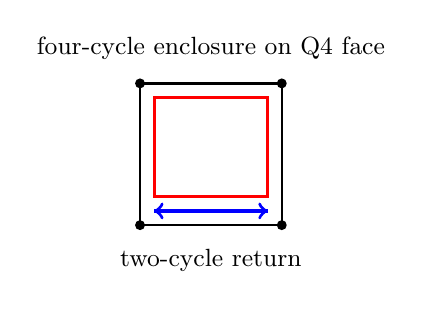
\begin{tikzpicture}[scale=0.9, every node/.style={font=\small}]
\coordinate (A) at (0,0); \coordinate (B) at (2,0); \coordinate (C) at (2,2); \coordinate (D) at (0,2);
\draw[thick] (A)--(B)--(C)--(D)--cycle;
\draw[very thick,blue,->] (0.2,0.2)--(1.8,0.2);
\draw[very thick,blue,->] (1.8,0.2)--(0.2,0.2);
\node at (1,-0.5) {two-cycle return};
\draw[very thick,red,->] (0.2,0.4)--(1.8,0.4)--(1.8,1.8)--(0.2,1.8)--cycle;
\node at (1,2.5) {four-cycle enclosure on Q4 face};
\fill (A) circle (2pt) (B) circle (2pt) (C) circle (2pt) (D) circle (2pt);
\end{tikzpicture}
\end{center}

\paragraph{Figure F2: $B^*$ ladder and attenuation.}
\begin{center}
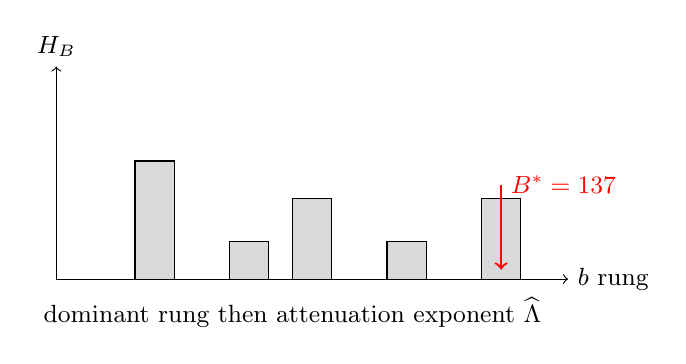
\begin{tikzpicture}[x=1cm,y=0.6cm, every node/.style={font=\small}]
\draw[->] (0,0) -- (6.5,0) node[right] {$b$ rung};
\draw[->] (0,0) -- (0,4.5) node[above] {$H_B$};
\draw[fill=gray!30] (1,0) rectangle +(0.5,2.5);
\draw[fill=gray!30] (2.2,0) rectangle +(0.5,0.8);
\draw[fill=gray!30] (3.0,0) rectangle +(0.5,1.7);
\draw[fill=gray!30] (4.2,0) rectangle +(0.5,0.8);
\draw[fill=gray!30] (5.4,0) rectangle +(0.5,1.7);
\draw[red,thick,->] (5.65,2) -- (5.65,0.2);
\node[red,right] at (5.65,2) {$B^*=137$};
\node at (3,-0.7) {dominant rung then attenuation exponent $\widehat\Lambda$};
\end{tikzpicture}
\end{center}

\paragraph{Figure F3: Collision / export-window diagram.}
\begin{center}
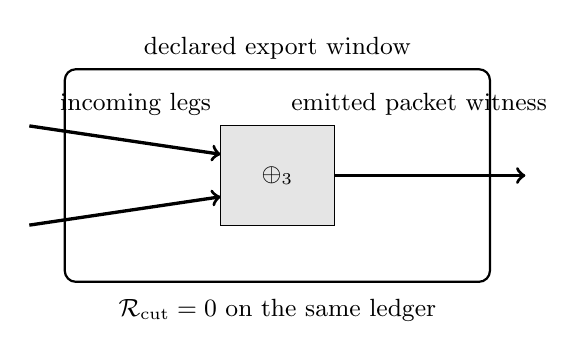
\begin{tikzpicture}[scale=0.9, every node/.style={font=\small}]
\draw[thick,rounded corners] (0,0) rectangle (6,3);
\node at (3,3.3) {declared export window};
\draw[->,very thick] (-0.5,2.2)--(2.2,1.8);
\draw[->,very thick] (-0.5,0.8)--(2.2,1.2);
\draw[fill=gray!20] (2.2,0.8) rectangle (3.8,2.2);
\node at (3,1.5) {$\oplus_3$};
\draw[->,very thick] (3.8,1.5)--(6.5,1.5);
\node at (1,2.5) {incoming legs};
\node at (5,2.5) {emitted packet witness};
\node at (3,-0.4) {$\mathcal R_{\mathrm{cut}}=0$ on the same ledger};
\end{tikzpicture}
\end{center}

\paragraph{Figure F4: Shell-band / cadence / torsion schematic.}
\begin{center}
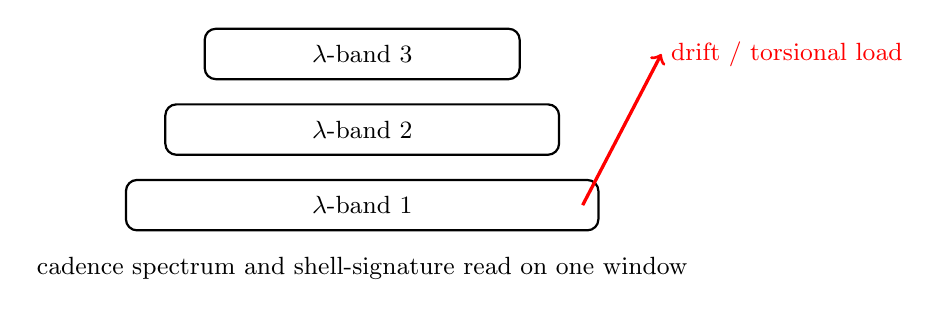
\begin{tikzpicture}[x=1cm,y=0.8cm, every node/.style={font=\small}]
\draw[thick,rounded corners] (0,0) rectangle (6,0.8);
\draw[thick,rounded corners] (0.5,1.2) rectangle (5.5,2);
\draw[thick,rounded corners] (1,2.4) rectangle (5,3.2);
\node at (3,0.4) {$\lambda$-band 1};
\node at (3,1.6) {$\lambda$-band 2};
\node at (3,2.8) {$\lambda$-band 3};
\draw[red,very thick,->] (5.8,0.4)--(6.8,2.8);
\node[red,right] at (6.8,2.8) {drift / torsional load};
\node at (3,-0.6) {cadence spectrum and shell-signature read on one window};
\end{tikzpicture}
\end{center}
